\chapter{Inferring the functional network corresponding to synchrony in the suprachiasmatic nucleus}
\blfootnote{Major portions of this chapter appear as
    J.H.\ Abel, K.\ Meeker, D.~Granados-Fuentes, P.C.\ St.~John, T.~Wang, B.\ Bales, F.J.\ Doyle~III, E.D.\ Herzog, and L.R.\ Petzold, ``Functional network inference of the suprachiasmatic nucleus,'' Proceedings of the National Academy of Sciences of the United States of America, vol.~113, no.~16, 2016. DOI:~10.10173/pnas.1521178113.
The discussion has been expanded to better fit the dissertation.
All statistical, modeling, and mathematical analyses were performed by J.H.\ Abel, with the exception of neuron tracking by B.\ Bales.
All experimental procedures were performed by members of the Herzog lab.
All writing was by J.H.\ Abel, except for the description of neuron tracking by B.\ Bales and experimental protocols by E.D.\ Herzog.
% copyright info: good to go http://www.pnas.org/site/aboutpnas/licenses.xhtml
}

\section{Introduction}
Neurons in the SCN generate circadian oscillations through a transcription-translation feedback loop, and are known to synchronize by the timely release of vasoactive intestinal peptide (VIP) and $\gamma$-aminobutyric acid (GABA) neurotransmitters which modulate the oscillator through the transcription factor CREB \cite{Aton2005,Albus2005, Welsh2010,Evans2013,DeWoskin2015}.
While the single-cell oscillator and coupling pathways have been extensively researched, relatively little is known about the structure of the neuronal network driving synchronization in the SCN. 
Prominent modeling studies of the past decade have assumed a wide variety of network structures: nearest neighbor \cite{To2007, An2013}, small-world \cite{Vasalou2009}, or mean-field \cite{Bernard2007, DeWoskin2014}; or combinations of these depending on coupling pathway \cite{DeWoskin2015}, pointing to the high degree of uncertainty regarding the general connectivity of the SCN.
There has been significant recent interest in attempting to elucidate the network structure and mechanisms driving synchrony the SCN, commonly through light-driven desynchronization assays \cite{Meijer2010, Evans2013, Evans2015, Myung2015}.
These methods have the advantage of reducing the SCN into large phase clusters of neurons, whose behavior can be easily tracked, and modeled with reduced approaches \cite{Myung2015}.
This approach has had great successes in reconciling the roles of GABA and VIP \cite{Albus2005, Evans2013, Myung2015, DeWoskin2015}.
A significant obstacle in developing a mechanistic understanding of synchronization in the SCN is the lack of single-cell resolution in these studies, preventing observation of the dynamics within these clusters.
Furthermore, light is received primarily by the core SCN, and this asymmetry of input is entangled with observed SCN behaviors \cite{Albus2005}.
Thus far, only fast-scale (phasic) GABA connections have been mapped at a single-cell resolution \cite{Freeman2013a}, and this phasic GABA release is not thought to affect the core oscillator \cite{DeWoskin2015}.


Here, we present a novel method for inferring the functional network of the suprachiasmatic nucleus during resynchronization at a single-cell resolution.
Our strategy involved the application of tetrodotoxin (TTX) to disperse single-cell phases through inhibition of intercellular coupling while allowing continued cell-autonomous oscillation \cite{Yamaguchi2003, Schwartz1987}. 
TTX was then washed out, restoring coupling and allowing reorganization of the SCN over the following eight days.  
We applied the maximal information coefficient (MIC) statistic \cite{Reshef2011} to bioluminescence recordings during resynchronization in order to identify ``functional connections'' within the SCN at a single-cell resolution.
Functional connections were defined between neurons which share a high degree of mutual information during resynchronization, characterized by a high MIC score.
Although functional connections connote neither causation nor direct physiological connection \cite{Eguiluz2005}, communication is necessary for SCN neurons to synchronize and maintain precise periodicity \cite{Herzog2004a}, resulting in a high mutual information between connected neurons.
We used this method to infer networks within five mouse SCN explants. 
Results showed that the suprachiasmatic nucleus has a consistent resynchronization network with a small-world topology and an exponential node degree distribution in each sample. 
The most densely connected neurons, or ``hubs,'' of each network were located in the central SCN.
Unlike prior studies involving phase clusters, a second cluster of connected shell neurons was not found.
Finally, we related our observed functional networks to the underlying physical network via stochastic simulation using two models of the coupled SCN \cite{Gonze2006,Schroder2012, Abel2015a}.

\section{Materials and methods}
\subsection*{Cell culture and bioluminescence recording}
SCN were obtained from 7-day old homozygous \textit{Per2$^{Luc}$} mice (founders generously provided by J. Takahashi, University of Texas Southwestern) housed under a 12h:12h light:dark schedule. 
All procedures were approved by the Washington University Animal Studies Committee and complied with NIH guidelines.
Bilateral SCN from 300 $\mu$m coronal sections of hypothalamus were cultured on Millicell-CM membranes (Millipore) in 400ml air-buffered Dulbecco's Modified Eagles Medium with two full-volume exchanges every 7 days.
After 14 days \textit{in vitro}, the culture was transferred to the stage of an inverted microscope (Nikon TE2000 fitted with a 20x objective and 0.5x coupler for a 10x magnification) inside a dark incubator (In Vivo Scientific).
We add 0.15mM beetle luciferin (BioThema) to the medium and imaged bioluminescence at 36$^\circ$C with an ultrasensitive CCD camera (Andor Ixon; 1x1 binning, 1 hour exposures).
Cultures were then treated with 2.5$\mu$M tetrodotoxin (TTX, Sigma) as previously described \cite{Webb2009}.
TTX remained in the medium for 6 days while imaging continued. We then performed three full-volume exchanges of fresh medium and resumed recording for 8-12 days to monitor resynchronization of \textit{Per2$^{Luc}$} rhythms.
Bright field images before and after each recording were used to focus and align the culture with prior images.

Software was developed to locate and track neuron bioluminescence intensities in each image time series.
In each frame, the software identified potential neurons using a standard difference of Gaussians blob detector.
The algorithm took the set of neuron locations in each image and attempted to find spatial correspondences between them in the image time series.
The correspondences were found by taking each potential neuron location and looking at previous images to find neurons in a nearby radius.
Because neurons could be undetectable for multiple frames (when bioluminescence is low), the search was extended back in time multiple frames with a slowly increasing search radius.
If the algorithm was able to connect a series of potential neuron locations through enough images, then it was assumed the sequence of locations represented a real neuron and the time series intensity was extracted from the images.
If the algorithm could not form a sufficiently long sequence of locations, the neuron was discarded as noise.
Results from automated neuron tracking were comparable to results obtained using manual tracking of neurons with ImageJ software \cite{Schneider2012}.

\subsection*{Numerical methods}
The MIC is calculated by partitioning a scatter plot of two variables ($X$ and $Y$; here, these are bioluminescence recordings from two cells) into an $n_x$-by-$n_y$ grid $g$ that maximizes mutual information $I_g(X;Y) = \sum_{y \in Y} \sum_{x \in X}
                 p(x,y) \log{ \left(\frac{p(x,y)}{p(x)\,p(y)}
                              \right) }$
normalized by the maximal mutual information, $\log\min\{n_x,n_y\}$, in $g$.
The optimal grid is selected as in \cite{Reshef2011}, by computing the normalized mutual information for a subset of all possible grids bounded in resolution by $n_x\times n_y<B$.
Details regarding this partitioning algorithm appear as Section 3 of the supplement to \cite{Reshef2011}.
As suggested in \cite{Reshef2011} we used binning parameter $B = N^{0.6}$, where $N$ is the number of data points in each time series. 
The MIC was calculated through the minepy package for Python (with interfaces to C++, R, MATLAB, and Octave) \cite{Albanese2013}.
The threshold for connectivity was selected based on receiver operating characteristic curves. 
Data analysis and processing was performed using Python. Network properties were calculated using the Networkx package \cite{Hagberg2008}.
Statistical tests for exponential and power law model fits were performed with the Python module powerlaw \cite{Alstott2014}, in a manner according to \cite{Clauset2009}. 
Numerical optimization (rather than a continuous approximation) was used to fit discrete exponential and power law (zeta) models, and a likelihood-ratio test was applied to determine goodness-of-fit.

Stochastic simulation of circadian models, as detailed in the following subsection, was performed in Python with the StochKit2 implementation of the Gillespie algorithm in the GillesPy (http://github.com/gillespy) library \cite{Sanft2011, Abel2017}.

\subsection*{Network simulations}

A stochastic three-state circadian oscillator with coupling through algebraic manipulation of \textit{Period} promotion \cite{Gonze2006, Schroder2012}, and a more detailed stochastic eleven-state circadian oscillator that explicitly captures VIP and CREB-based \textit{Period} promotion for coupling \cite{Abel2015a} were selected for our simulations.
The degree of stochasticity or noise within these models was fit as in \cite{Rougemont2007, StJohn2014b}: we captured the noise strength by tuning the volume parameter $\Omega$ for the stochastic models to fit the desynchronization rate for a population of uncoupled oscillators.
This also captures the distribution of period lengths driven by intrinsic stochasticity \cite{StJohn2015}.
Each cell within these networks was parameterized identically to reflect the primary importance of intrinsic variability in SCN neurons \cite{Herzog2004a}, and to ensure that this inference method can distinguish between connected and unconnected cells even in the case where all other parameters (amplitude, mean period, phase angle, noise intensity) are identical.
Full equations and parameter sets for these simulations are included below.

Network resynchronization simulations were designed to reproduce the TTX-mediated resynchronization experiments.
A population of cells, initially at an identical phase, was simulated stochastically with no coupling and allowed to desynchronize for six days, to mimic TTX inhibition of intercellular communication.
Amplitude damping (as in the experiment) is observed only in the eleven-state model, due to the more mechanistically accurate coupling terms.
After six days, coupling was restored with a predetermined network topology and simulation continued for an additional eight days.
\textit{Per} mRNA count was recorded in one-hour simulation intervals to reflect bioluminescence counts with one sample per hour.
The MIC statistic was calculated as for the experimental data, using the resulting \textit{Per} mRNA traces rather than bioluminescence.
Representative simulations of the three-state and eleven-state models are shown in the following section.


\begin{table}[p]
\caption{\label{tab:s1}Ordinary differential equations and parameters comprising the three-state circadian model \cite{Gonze2006}.
    For these equations $j$ indicates the index of the current cell, $i$ indicates the indexes of cells coupled to cell $j$, and $I$ is the total number of cells coupled to cell $j$.}
\vspace{0.5cm}
\begin{center}
{
\begin{tabular}{l l l}\hline
	State Variable & Symbol & Conservation Equation\\
	\hline\\
	mRNA & \textbf{M} & $\displaystyle\frac{d\mathbf{M}}{dt} = 
	v_s\frac{K_1^n}{K_1^n + \mathbf{PN}^n} 
	- \frac{v_m\mathbf{M}}{K_m+\mathbf{M}}
	$\\[0.6cm]
	Cytosolic protein & \textbf{PC} & $\displaystyle\frac{d\mathbf{PC}}{dt} 
	= k_s\mathbf{M} - \frac{v_d\mathbf{PC}}{K_d + \mathbf{PC}} 
	- k_1\mathbf{PC} + k_2\mathbf{PN}
	$\\[0.6cm]
	Nuclear protein & \textbf{PN} & $\displaystyle\frac{d\mathbf{PN}}{dt} 
	= k_1\mathbf{PC} - k_2\mathbf{PN}
	$\\[0.6cm]
    \hline
\end{tabular}\\[1em]
\begin{tabular}{l l l l}\hline
	Parameter & Description & Value & Units\\
	\hline\\
	$v_s^0$ & Minimum mRNA transcription rate & 0.82 & [-]/hr\\
	$w$ & Weighting of connected cells & 0.0050 & Dimensionless \\
	$a$ & Coupling strength & 2 & 1/hr\\
	$c_j$ & Coupling term for cell $j$ &  
	$a\bigg(\frac{\mathbf{M_j} + w\sum \mathbf{M_i}}{1+
	I\times w} -\mathbf{M_j}\bigg)$\\
	$v_s$ & mRNA transcription rate & $\displaystyle v_s^0 + c_j$ 
	& [-]/hr \\
	$n$ & mRNA transcription Hill term & 4.0 & Dimensionless\\
	$K_1$ & mRNA transcription constant & 1.0 & [-]\\
	$v_m$ & mRNA degradation rate & 0.42 & [-]/hr\\
	$K_m$ & mRNA degradation constant & 0.50 & [-]\\
	$k_s$ & Protein translation rate & 0.42 & 1/hr\\
	$v_d$ & Cytosolic protein degradation rate & 1.2 & [-]/hr\\
	$K_d$ & Cytosolic protein degradation constant & 0.13 & [-]\\
	$k_1$ & Cytosolic to nuclear protein rate & 0.42  & 1/hr\\
	$k_2$ & Nuclear to cytosolic protein rate & 0.50 & 1/hr\\
	\hline
\end{tabular}
}
\end{center}
\end{table}


\begin{table}[p]
    \caption{\label{tab:s2}
    Ordinary differential equations and parameters comprising the 11-state circadian model \cite{Abel2015a}, continued on following page.}
\begin{center}
\begin{tabular}{l l l}\hline
	State Variable & Symbol & Conservation Equation\\
	\hline\\
	\textit{Per} mRNA & \textbf{p} & $\displaystyle\frac{d\mathbf{p}}{dt} = \frac{v_{1pp}\mathbf{CREB} + v_{2pr}}{K_{1p} + \mathbf{C1P}+ \mathbf{C2P}} - \frac{v_{3p}\mathbf{p}}{K_{2dp}+\mathbf{p}}$
	\\[0.4cm]
	\textit{Cry1} mRNA & \textbf{c1} & $\displaystyle\frac{d\mathbf{c1}}{dt} = \frac{v_{4c1r}}{K_{3c} + \mathbf{C1P}+ \mathbf{C2P}} - \frac{v_{5c1}\mathbf{c1}}{K_{4dc}+\mathbf{c1}}
$ 
	\\[0.4cm]
	\textit{Cry2} mRNA & \textbf{c2} & $\displaystyle\frac{d\mathbf{c2}}{dt} = \frac{v_{6c2r}}{K_{3c} + \mathbf{C1P}+ \mathbf{C2P}} - \frac{v_{7c2}\mathbf{c2}}{K_{4dc}+\mathbf{c2}}
$ 
	\\[0.4cm]
	\textit{VIP} mRNA & \textbf{vip} & $\displaystyle\frac{d\mathbf{vip}}{dt} = \frac{v_{8vr}}{K_{5v} + \mathbf{C1P}+ \mathbf{C2P}} - \frac{v_{9v}\mathbf{vip}}{K_{6dv}+\mathbf{vip}}
$ 
	\\[0.4cm]
	\textit{Per} Protein & \textbf{PER} & \splitcell{
		$\displaystyle\frac{d\mathbf{P}}{dt} = k_{1p}\mathbf{p} - \frac{v_{10P}\mathbf{P}}{K_{7dP}+\mathbf{P}} - v_{11aCP}\mathbf{P}\times\mathbf{C1}- v_{11aCP}\mathbf{P}\times\mathbf{C2}$\\[0.3cm] $\;\;\;\;\;\;\;\; + v_{12dCP}\mathbf{C1P} + v_{12dCP}\mathbf{C2P}
	$ }
	\\[0.4cm]
	\textit{Cry1} Protein & \textbf{C1} & $\displaystyle\frac{d\mathbf{C1}}{dt} = k_{2c}\mathbf{c1} - \frac{v_{13C1}\mathbf{C1}}{K_{8dC}+\mathbf{C1}} - v_{11aCP}\mathbf{P}\times\mathbf{C1} + v_{12dCP}\mathbf{C1P}
$ 
	\\[0.4cm]
	\textit{Cry2} Protein & \textbf{C2} & $\displaystyle\frac{d\mathbf{C2}}{dt} = k_{2c}\mathbf{c2} - \frac{v_{14C2}\mathbf{C2}}{K_{8dC}+\mathbf{C2}} - v_{11aCP}\mathbf{P}\times\mathbf{C2} + v_{12dCP}\mathbf{C2P}
$ 
	\\[0.4cm]
	\textit{VIP} Protein & \textbf{VIP} & $\displaystyle\frac{d\mathbf{VIP_j}}{dt} = k_{3v}\sum\limits_{i}^I w_i\mathbf{vip_i} - v_{15V}\mathbf{VIP_j}
$ 
	\\[0.4cm]
    CRY1-PER Dimer & \textbf{C1P} & $\displaystyle\frac{d\mathbf{C1P}}{dt} = v_{11aCP}\mathbf{P}\times\mathbf{C1} - v_{12dCP}\mathbf{C1P} - \frac{v_{16C1P}\mathbf{C1P}}{K_{9dCn}+\mathbf{C1P} + \mathbf{C2P}}
$ 
	\\[0.4cm]
	CRY2-PER Dimer & \textbf{C2P} & $\displaystyle\frac{d\mathbf{C2P}}{dt} = v_{11aCP}\mathbf{P}\times\mathbf{C2} - v_{12dCP}\mathbf{C2P} - \frac{v_{17C2P}\mathbf{C2P}}{K_{9dCn}+\mathbf{C1P} + \mathbf{C2P}}
$ 
	\\[0.4cm]
	CREB Protein & \textbf{CREB} & $\displaystyle\frac{d\mathbf{CREB}}{dt} = \frac{v_{18V}\mathbf{VIP}}{K_{10V}+\mathbf{VIP}} - \frac{v_{19CR}\mathbf{CREB}}{K_{11dCR}+\mathbf{CREB}}
$\\[0.4cm] 
\hline
\end{tabular}
\end{center}
\end{table}


\begin{table}[p]
\contcaption{(Continued.)}
    \begin{center}
\begin{tabular}{l l l l}\hline
	Parameter & Description & Value & Units\\
	\hline
	$v_{1pp}$ & CREB-induced \textit{Per} mRNA promotion & 0.235 & [-]/hr
	\\
	$v_{2pr}$ & \textit{Per} mRNA transcription & 0.415 & [-]$^2$/hr
	\\
	$v_{3p}$ & \textit{Per} mRNA degradation & 0.478 & [-]/hr
	\\
	$v_{4c1r}$ & \textit{Cry1} mRNA transcription & 0.350 & [-]$^2$/hr
	\\
	$v_{5c1}$ & \textit{Cry1} mRNA degradation & 1.44 & [-]/hr
	\\
	$v_{6c2r}$ & \textit{Cry2} mRNA transcription & 0.124 & [-]/hr
	\\
	$v_{7c2}$ & \textit{Cry2} mRNA degradation & 2.28 & [-]/hr
	\\
	$v_{8vr}$ & \textit{VIP} mRNA transcription & 0.291 & [-]$^2$/hr
	\\
	$v_{9v}$ & \textit{VIP} mRNA degradation & 1.35 & [-]/hr
	\\
	$v_{10P}$ & \textit{Per} protein degradation & 13.0 & [-]/hr
	\\
	$v_{11aCP}$ & PER-CRY dimer formation & 0.493 & ([-]$\times$ hr)$^{-1}$
	\\
	$v_{12dcp}$ & PER-CRY dimer dissociation & 0.00380 & 1/hr
	\\
	$v_{13C1}$ & \textit{Cry1} protein degradation & 4.12 & [-]/hr
	\\
	$v_{14C2}$ & \textit{Cry2} protein degradation & 0.840 & [-]/hr
	\\
	$v_{15V}$ & \textit{VIP} protein degradation & 0.723 & 1/hr
	\\
	$v_{16C1P}$ & PER-CRY1 dimer degradation & 0.0306 & [-]/hr
	\\
	$v_{17C2P}$ & PER-CRY2 dimer degradation & 0.0862 & [-]/hr
	\\
	$v_{18V}$ & CREB activation by VIP receptors & 0.789 & [-]/hr
	\\
	$v_{19CR}$ & CREB deactivation & 1.27& [-]/hr
	\\
	$k_{1p}$ & PER translation & 7.51 & 1/hr	
	\\
	$k_{2c}$ & CRY translation & 0.572 & 1/hr
	\\
	$k_{3v}$ & VIP translation & 5.50 & 1/hr
	\\
	$K_{1p}$ & \textit{Per} transcription constant & 0.264 & [-]
	\\
	$K_{2dp}$ & \textit{Per} degradation constant & 0.00795 & [-]
	\\
	$K_{3c}$ & \textit{Cry} transcription constant & 0.156 & [-]
	\\
	$K_{4dc}$ & \textit{Cry} degradation constant & 1.94 & [-]
	\\
	$K_{5v}$ & \textit{VIP} transcription constant & 0.115 & [-]
	\\
	$K_{6dv}$ & \textit{VIP} degradation constant & 0.110 & [-]
	\\
	$K_{7dP}$ & \textit{Per} protein degradation constant & 0.0372 & [-]
	\\
	$K_{8dC}$ & \textit{Cry} protein degradation constant & 4.23 & [-]
	\\
	$K_{9dCn}$ & PER-CRY dimer degradation constant & 0.0455 & [-]
	\\
	$K_{10V}$ & CREB protein activation constant & 1.46 & [-]
	\\
    $K_{11CR}$ & CREB protein deactivation constant & 1.01 & [-]
    \\[0.0cm]
	\hline
\end{tabular}
\end{center}
\end{table}


\subsection*{Circadian models and parameters}
\label{sub:models}
Table \ref{tab:s1} contains the equations and parameters for the three-state model of the mammalian circadian oscillator \cite{Gonze2006, Schroder2012}.
Coupling is achieved in this model through the modulation of mRNA production rate, $v_s$.
A cell with index $j$ transcribes mRNA with maximum rate $v_s = v_s^0 +c_j$, where $v_s^0$ is the baseline maximum rate and $c_j$ is the coupling term, which is dependent on the mRNA concentrations of connected cells.
The coupling term $c_j$ is bounded at 0. 
This reflects the fact that intercellular coupling is accomplished through \textit{Per} promotion.
To simulate stochastically, biomolecule concentrations were converted to populations, through use of a volume parameter, $\Omega$. For this model, $\Omega = 40$ captured the correct degree of stochasticity as calculated in \cite{Rougemont2007, StJohn2014b}.

Table \ref{tab:s2} contains the equations and parameters for the eleven-state model \cite{Abel2015a}.
In this model, coupling between neuron 1 and neuron 2 is achieved by VIP mRNA from neuron 1 being directly translated into VIP protein affecting cell 2, and vice-versa.
So that each cell receives the same total VIP input (to keep the model consistent), the VIP input is weighted by the total number of connections $C$.
The weighting parameter $w_i$ is therefore equal to $1/C$ for each connected cell.
In this model, the volume parameter $\Omega$ was set to 400, as in \cite{Abel2015a}.

For each model, cells which were not found to have functional connections were simulated with a weakened coupling to the mean field, to reflect the fact that these cells do eventually synchronize.
This could be biologically indicative of weak coupling pathways, or simply that we did not detect their strong connections, as they did not exceed our threshold.
For the three-state model, this was achieved by mean-field coupling with a weight parameter $w=0.0025$.
For the eleven state model, this was accomplished by mean-field VIP input with coupling strength $w_{i,weakfield}=0.25k_{3v}$ and additional VIP input from the uncoupled cell itself $w_{i,self}=0.75k_{3v}$ such that each cell receives an input of identical strength.








\section{Results}
\subsection*{Design of resynchronization experiment}

\begin{figure}[p]
    \begin{center}
        \includegraphics[width=3.5in]{chap3/figures/fig1.pdf}
    \end{center}
    \caption{\label{fig:expt}Experimental protocol demonstrating TTX-mediated resynchronization for SCN1. (\textbf{A}) Bioluminescence traces from individual cells within SCN1, showing pre-TTX, during-TTX, and post-TTX single-cell oscillations. 
    (\textbf{B}) In the functioning SCN, peak times are highly correlated from cycle to cycle. We compare relative peak times 1 (pre-TTX), 2 (during-TTX), and 3-4 (post-TTX), to the first peak (0) in order show that a resynchronization is indeed taking place, and that the SCN network structure reverts to pre-TTX structure slowly after TTX wash.
   (\textbf{C}) Plot of Pearson $r$ for correlating each peak to peak 0, showing the resynchronization. Pearson $r$ does not completely return to pre-TTX levels due to inability to track cells accurately across TTX conditions.}
\end{figure}



To infer the SCN network, we observed five whole SCN mouse explants resynchronizing after decoupling by tetrodotoxin (TTX) (Figure \ref{fig:expt}).
\textit{Per2$^{Luc}$} knock-in SCN explants were cultured while under a microscope, allowing the capture of single-cell bioluminescence within the whole SCN.
Bioluminescence counts were recorded each hour, and individual neurons were identified and tracked manually from the resulting images.
These single-cell traces are shown in Figure \ref{fig:expt}A for SCN1.
TTX was applied to the whole tissue explants for six days to inhibit intercellular coupling, while leaving physical connections within the tissue intact \cite{Yamaguchi2003, Webb2009, Buhr2010}.
After six days, the TTX was washed out, and recordings continued for an additional 8 days as neurons in the network regained synchrony.
In the synchronized SCN there was a strong correlation from cycle to cycle for single-cell relative peak times\cite{Yamaguchi2003}.
We demonstrate the loss of this hierarchy during TTX application and its restoration after TTX washout in Figure \ref{fig:expt}B.
Pearson's $r$ is shown for correlations between peak 0 pre-TTX, and peaks 1-4 at different experimental stages.
By day 5 of TTX application (peak 2), all correlation with peak 0 was effectively removed.
Shortly after TTX washout some correlation was restored, and correlation was completely restored by peak 4 (day 7 post-TTX).
In Figure \ref{fig:expt}C, correlation with peak 0 for each day is shown.
The restoration of correlation in peak times between pre- and post-TTX regions indicated that the original pre-TTX hierarchy was slowly restored over the course of several days post-TTX.
Pearson's $r$ returned to a maximum of $\sim 0.7$ due to imperfect cell tracking between pre-, during-, and post-TTX conditions.
Approximately 40\% of cells in each SCN explant lost observable rhythmicity during TTX application, corresponding with \cite{Webb2009}.
These cells were not included in this figure although they were included in the bioluminescence traces from the post-TTX resynchronization period used to infer network connectivity.
A summary of rhythmcity, period distribution, and noise is included as Figure \ref{fig:s1}.
This protocol resulted in ensembles of single-cell resynchronization traces from five biologically distinct SCNs each containing approximately 400 cells.
This dataset is publicly available online at https://github.com/JohnAbel/scn-resynchronization-data-2016.
\afterpage{
\begin{figure}[p]
    \caption{\label{fig:s1} 
Summary statistics for SCN slices during TTX application and during resynchronization.
    (\textbf{A, D}) Fraction of cells which displayed rhythmic circadian oscillation (A) during TTX or (D) during resynchronization. Not all cells observed during resynchronization could be tracked during TTX due to very low luminescence (as in \cite{Webb2009}); cells which could not be tracked were classified as arrhythmic. We found that chemically uncoupled cells are nondeterministic, weak oscillators, in accordance with \cite{Webb2009}. When re-coupled after TTX washout, nearly all cells observed became rhythmic. A cell was determined to be rhythmic if it exhibited a Lomb-Scargle periodogram peak between 18-32h period at $P<0.05$ significance. Data was baseline detrended via discrete wavelet transform.
    (\textbf{B, E}) Period length histograms (B) during TTX application and (E) during resynchronization. As period varies cycle-to-cycle for decoupled oscillators and during resynchronization, we report each peak to peak period of oscillation for each cell, rather than finding the mean period of a cell through fitting a sinusoid. Peak times were identified by a discrete wavelet transform filtering for peaks with period between 16-32h.
    (\textbf{C, F}) Histograms of the fraction of oscillatory power in the circadian frequency range (16-32h) (C) during TTX or (F) during resynchronization, calculated via fast Fourier transform. Data was baseline detrended before FFT. We note that not all cells are observable during TTX due to low bioluminescence, and thus column (C) includes only rhythmic, observable cells. For all SCNs, the period distribution tightened and more oscillatory power was in the circadian range during resynchronization. As these effects and distributions are consistent across SCNs during resynchronization, a cross-comparison may be used to control false positive rate.
}
\end{figure}
\begin{figure}[p]
    \begin{center}
        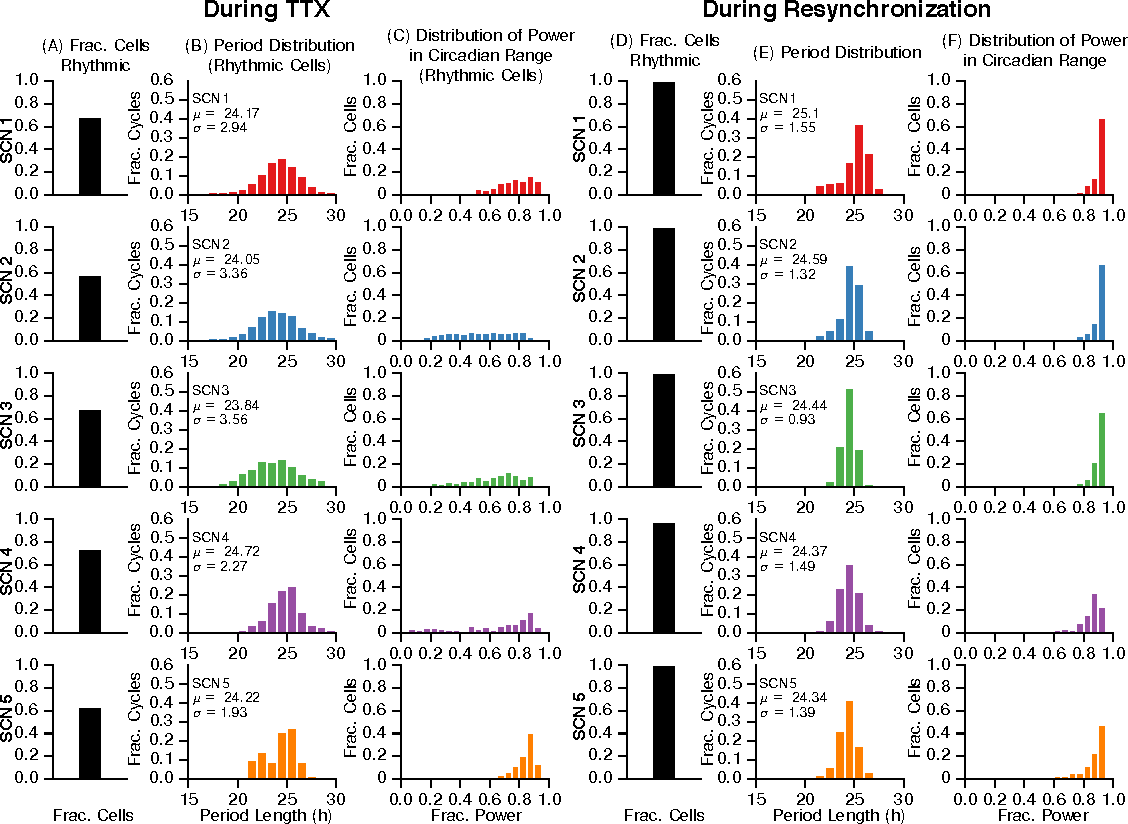
\includegraphics[width=6.5in]{chap3/figures/s1.pdf}
    \end{center}
    \contcaption{(Continued.)}
\end{figure}
}


\subsection*{Inferring connections between SCN neurons}

While fast-scale and electrical connections between individual neurons have been identified by methods such as mutual information, transfer entropy, directed transfer functions, Granger causality, or between-sample analysis of connectivity (BSAC) \cite{Garofalo2009, Bettencourt2007, Kaminski2001, Pourzanjani2015, Freeman2013a}, these methods are not suitable here due to nonstationary gene expression and the slow-scale nature of VIP and GABA feedback to the core oscillator, resulting in the damping of high-frequency signals \cite{Fujita2010, Pourzanjani2015, DeWoskin2015}.
High frequency GABA signals affect the firing of SCN neurons, and have been mapped previously \cite{Freeman2013a}, however, fast scale GABA is not thought to affect the core oscillator \cite{DeWoskin2015}.
Additionally, due to the limitations of the \textit{Per2$^{Luc}$} bioluminescent reporter used to observe core clock gene expression, the most rapid sampling provides 30 minute sample intervals \cite{Evans2013}, insufficient for methods such as Granger causality \cite{Pourzanjani2015}.

We inferred connections within these samples using the maximal information coefficient (MIC) as our correlation metric \cite{Reshef2011}.
MIC is effectively a continuous metric of mutual information, and is calculated by partitioning a scatter plot of two variables (in this case, raw bioluminescence recordings of two cells) in phase space into a grid that maximizes the mutual information.
We selected this statistic because it readily captures relationships between noisy continuous random variables.
MIC scores are high between cells which have identical periods and precise phase relationships, which is indicative of communication to resist the stochastic phase drift that occurs in uncoupled neurons.
Strongly or directly connected cells will drift apart less in phase and have more precise periodicity than cells which are unconnected.
This point, and the effects of sampling rate, cell amplitudes, and noise on MIC scores are examined via stochastic simulation in Figures \ref{fig:s2} and \ref{fig:s3}.
Because MIC partitions each pair of variables onto a grid, and computes the density of grid regions, it effectively performs a normalization of oscillation amplitude: scaling the amplitude of one or both cells will not affect the pairwise MIC score.
Notably, MIC shows a bias toward oscillatory states with a small phase offset.
To account for this, we repeated the entirety of the following analyses with a phase correction for each cell pair, and show that our results are consistent (following the main results, Figure \ref{fig:s4}).

\begin{figure}[p]
    \caption{\label{fig:s2} 
    MIC score for identification of network connections is largely invariant with respect to sampling rate and amplitude (continued from previous page).
In A-C, we test the effect of sampling rate on the ability to distinguish between strongly and weakly coupled simulated cells.
We use strongly and weakly coupled cells rather than coupled and uncoupled cells because the entire SCN is indirectly coupled, and therefore we are only interested in the strongest connections.
In D-E, we show that the MIC binning procedure effectively normalizes amplitude, and therefore raw amplitude has no effect on MIC score.
(\textbf{A}) Per mRNA traces for two weakly coupled cells (left, coupling strength parameter = 0.0033) and two strongly coupled cells (right, coupling strength parameter = 0.010). For both simulations in A-C, the discrete stochastic three-state model \cite{Schroder2012} was used, with volume parameter $\Omega$ = 40, and the simulation sampling rate was set to 100 samples per hour.
(\textbf{B}) Scatter plots and MIC values of Per mRNA for the cell pairs, downsampled to 1 hour intervals, or 6 hour intervals.
(\textbf{C}) Effect of sample interval on MIC score. For sampling intervals shorter than approximately 2h, only marginal changes in MIC are seen, indicating that the MIC score is largely consistent with increased sampling rate.
For sampling intervals longer than 2h (fewer than 10 samples/cycle), the MIC score becomes less accurate, and the ability to distinguish between connections of varying strength is reduced.
(\textbf{D}) To demonstrate the effective normalization of cellular trajectories through MIC binning, we compared MIC values for strongly and weakly coupled cells, while scaling the peak-to-trough amplitude.
    For both simulations in D-E, the sampling rate was set to 1 sample per hour. Peak to trough amplitude of one of the resulting trajectories was scaled to $Amp = 10$ (top) or $Amp = 500$ (bottom) for visualization.
    (\textbf{E}) MIC score is completely invariant with respect to changes in amplitude of a simulated trajectory, as the gridding algorithm in MIC is effectively a normalization.
}
\end{figure}
\begin{figure}[p]
    \begin{center}
        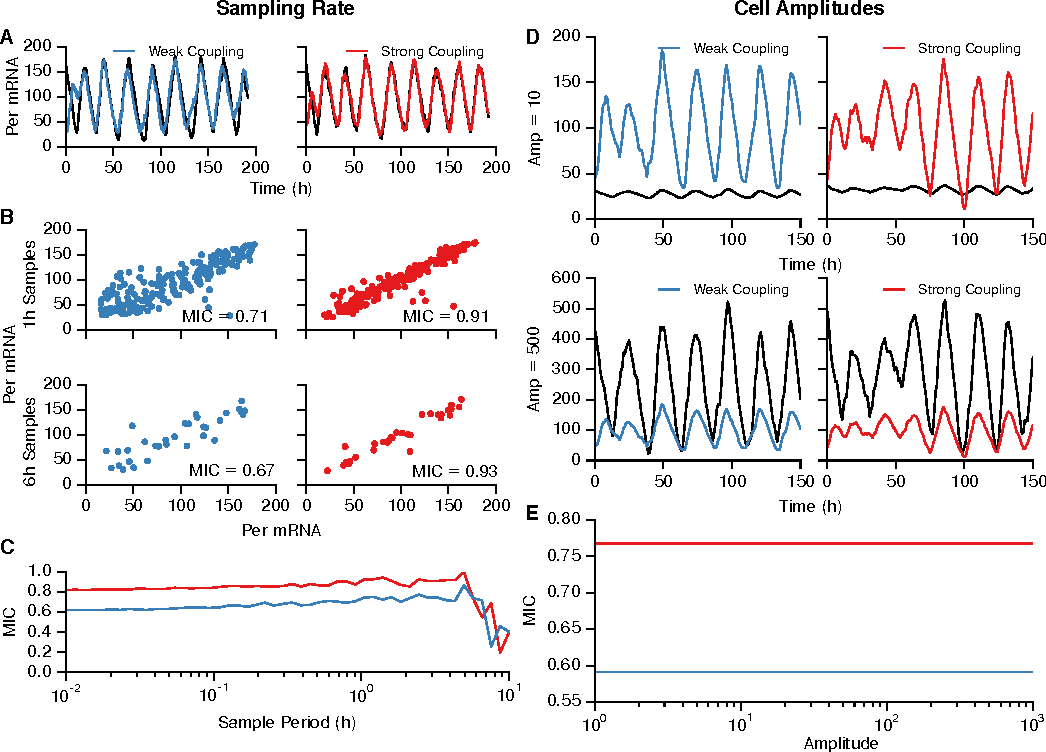
\includegraphics[width=6.5in]{chap3/figures/s2.pdf}
    \end{center}
\contcaption{(Continued.)}
\end{figure}





\begin{figure}[p]
    \begin{center}
        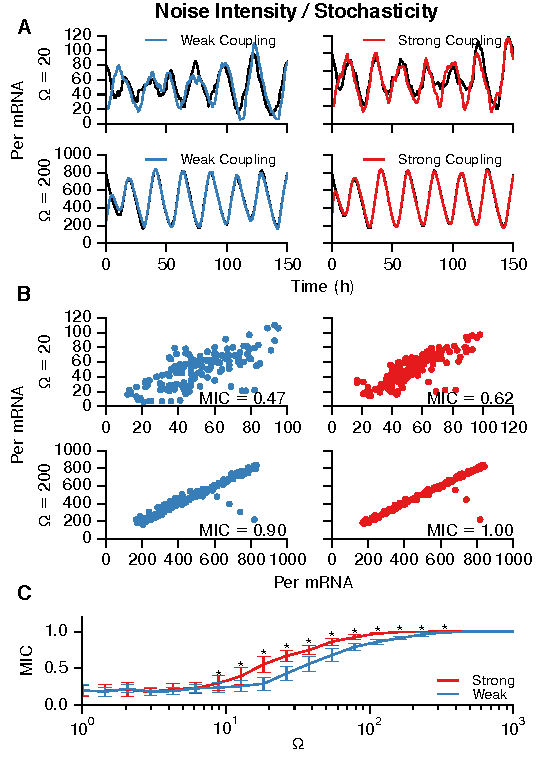
\includegraphics[width=3.5in]{chap3/figures/s3.pdf}
    \end{center}
    \caption{\label{fig:s3} 
    MIC is able to distinguish between strongly and weakly connected cells for a wide range of stochasticity. Stochastic noise in the three-state model \cite{Schroder2012} was tuned by changing the volume parameter $\Omega$.
    Stochastic noise causes cells to drift in phase, and thus is essential for this inference.
    (\textbf{A}) Representative Per mRNA traces of weakly coupled (left, coupling strength = 0.0033) and strongly coupled (right, coupling strength = 0.010) cells resynchronizing for $\Omega=20$ (top) and $\Omega=200$ (bottom). For all simulations here, sampling intervals were 1h, as in the experiment.
    (\textbf{B}) Scatter plots and MIC values of Per mRNA for these representative cell pairs at $\Omega=20$ and $\Omega=200$.
    (\textbf{C}) Plot of mean $\pm$ S.D. MIC values for strongly and weakly coupled cell pairs vs. $\Omega$ (n = 33 cell pairs at each $\Omega$). A broad range of stochasticity allows differentiation between strong and weak coupling ($^\star$P$ < 0.05$, Wilcoxon sign rank test with Bonferroni correction).
    At very low $\Omega$ values, oscillation does not occur, and at very high $\Omega$ values, the MIC scores for both pairs approach 1.0. The experimentally-determined $\Omega = 40$ is well within the range for which MIC can distinguish between connections.
}
\end{figure}







\begin{figure}[p]
    \begin{center}
        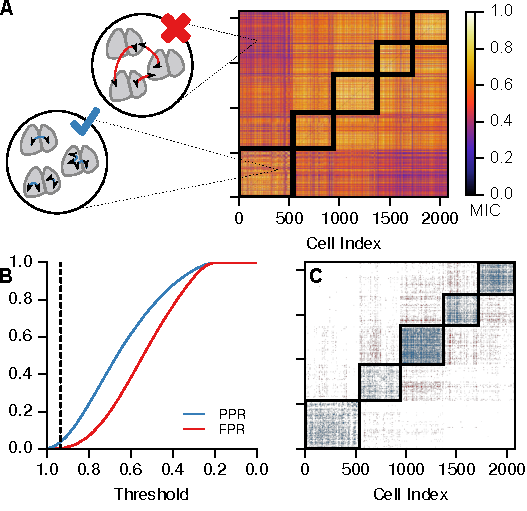
\includegraphics[width=3.5in]{chap3/figures/fig2.pdf}
    \end{center}
    \caption{\label{fig:ctrl}MIC identifies the strongest connections within a whole SCN sample.
	(\textbf{A}) Here, we calculate and plot pairwise MIC between neurons from all SCNs. We consider connections within the same SCN to be valid, whether between halves or within a single half. Connections between physiologically-distinct SCNs are invalid, as they are biologically infeasible. The block-diagonal regions outlined in black contain valid connections, and connections outside of this region are invalid.  
    (\textbf{B}) False positive rate (FPR, red, inter-SCN connections) and possible positive rate (PPR, blue, same-SCN connections) are plotted for varying MIC threshold values. We choose an initial threshold of 0.935, for which FPR $= 0.0032$.
    (\textbf{C}) The connections identified by applying the threshold from (B) are shown to occur primarily in biologically-valid areas (blue), with few invalid connections found (red). Thus, the strongest functional connections within each SCN are identified.
}
\end{figure}




We applied this correlation metric to pairs of bioluminescence traces from cells from all five SCNs. 
No detrending or other pre-processing was performed on this data.
MIC was calculated using raw bioluminescence of each pair of cells.
We then used a receiver operating characteristic (ROC) curve to determine if the method can differentiate between biologically distinct SCNs, and to establish a MIC connectivity threshold that rejects known false positives (Figure \ref{fig:ctrl}). 
SCN mean phases were aligned before computing MIC for this negative control in order to prevent biases due to misaligned phase.
These five SCNs were cultured separately and bear no common influences, thus no connections should be found between them. 
A ``possible positive'' was defined to be an inferred connection within the same SCN (Figure \ref{fig:ctrl}A), whereas a false positive was a
biologically-impossible inferred connection between two different SCNs. 
As it is only known \textit{a priori} which connections cannot exist, we calculated a possible positive rate (PPR, connections within the same SCN) and false positive rate (FPR, connections between biologically-distinct SCNs), to validate that MIC preferentially detects physiologically-valid connectivity.

To infer the network structure within the SCN, we selected a critical MIC  parameter, $m_{crit}$, from this control result.  
Pairs of cells that have a MIC score above $m_{crit}$ were determined to be functionally connected.
Our $m_{crit}$ threshold was chosen to be $0.935$, as 
this value has a $0.0032$ FPR, while still capturing the strongest connections with PPR $= 0.036$.
To account for slight variations in rate of synchronization between SCNs, we adjusted this threshold above $m_{crit}$ for each SCN to normalize average node degree (average number of connections per cell) between networks.
Because threshold values were raised, this results in a more conservative estimate of connectivity.
For SCNs 1-5, threshold values were raised to 0.949, 0.935, 0.990, 0.968, and 0.969 to yield average node degrees or 4.44, 4.49, 3.94, 4.80, and 4.56, respectively. 

\subsection*{SCN functional network displays a small-world exponential architecture}

\begin{figure}[p]
    \begin{center}
        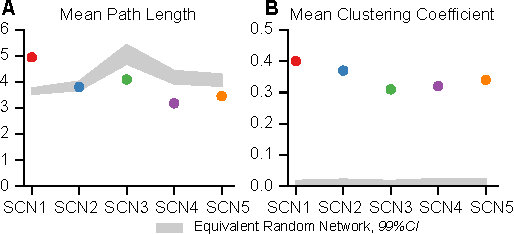
\includegraphics[width=3.5in]{chap3/figures/fig3.pdf}
    \end{center}
    \caption{\label{fig:mcs} SCN functional networks display small-world structure. (\textbf{A}) Average path length is on the same order of magnitude of an equivalent random (Erdos-Renyi) network. (\textbf{B}) Clustering coefficient is a magnitude greater than that of equivalent randomly-generated networks. Confidence intervals determined by generation of 10,000 equivalent Erdos-Renyi networks for each SCN.
}
\end{figure}


Networks inferred from the five SCN explants exhibit small-world characteristics as shown in Figure \ref{fig:mcs}.
Small-world networks are commonly found in biological systems, and are identified by the average path length $L$ and clustering coefficient $C^\Delta$, as defined in \cite{Watts1998, Newman2000}.
A network $G$ is determined to be small world if the average path length of $G$, $L_G$, is similar to the average path length $L_{rand}$ for the equivalent random graph, and the clustering coefficient $C^\Delta_G$ is an order of magnitude greater than $C^\Delta_{rand}$. That is:
\begin{equation} 
	L_{G} \approx L_{random} \; 
	\mbox{and} \; 
	C^{\Delta}_{G} \gg C^\Delta_{random}  \mbox{,}
\end{equation} 
where the equivalent random graph has the same number of vertices and edges.
As shown in Figure \ref{fig:mcs}, each SCN met the criteria for small-world architecture.
Confidence intervals shown for random networks are determined by generation of 10,000 Erdos-Renyi equivalent networks for each SCN.
Figure \ref{fig:s5} demonstrates that these network characteristics are consistent across SCNs, and locally insensitive to the choice of connectivity threshold.

\afterpage{\clearpage
\begin{table}[p]				
	\label{tab:swn}	
	\caption{\textbf{SCN Network Characteristics} Threshold, average node degree (average connections per cell $k$), average path length $L$ (average number of steps between cells in the network), and average clustering coefficient C$^\Delta$ 
\cite{Watts1998, Newman2000}
      of SCN networks.		
  Average path length, and clustering coefficient for SCNs 1-5 show agreement and small-world network characteristics (high clustering coefficient).		
  Connectivity threshold was raised above $m_{crit}$ from Figure 2B to yield $ND \sim 4.5$ for each SCN.}	
    \begin{center}		
  \begin{tabular}{lllll}		
\hline		
 Network & Threshold & Avg. $k$ & Avg. $L$ & Avg. C$^\Delta$ \\		
 \hline		
 SCN1    & 0.949     & 4.44         & 4.95             & 0.40                   \\		
 SCN2    & 0.935     & 4.49         & 3.81             & 0.37                   \\		
 SCN3    & 0.990     & 3.94         & 4.10             & 0.31                   \\		
 SCN4    & 0.968     & 4.80         & 3.18             & 0.32                   \\		
 SCN5    & 0.969     & 4.56         & 3.46             & 0.34                   \\		
\hline		
\end{tabular}
    \end{center}		
  \bigskip		
\end{table}
\clearpage
}

\begin{figure}[p]
    \begin{center}
        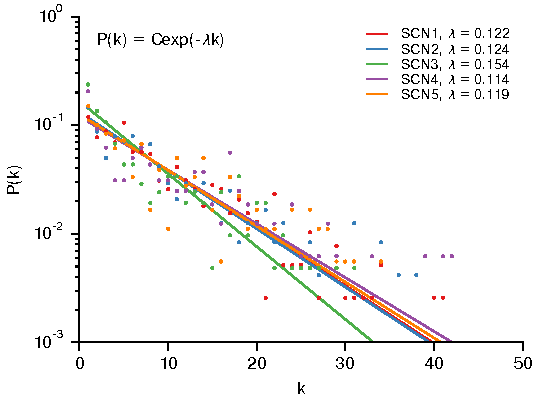
\includegraphics[width=3.5in]{chap3/figures/fig4.pdf}
    \end{center}
    \caption{\label{fig:log} Node degree ($k$) distributions for SCNs 1-5 plotted on a semilog scale. The resulting discrete exponential distributions $P(k) = C\exp(-\lambda k)$ were fit via numerical optimization of the maximum likelihood, resulting in distribution parameters $\lambda$ for each network. Each SCN is better fit by a discrete exponential distribution than a discrete power law distribution (likelihood-ratio test, $P<0.0005$ for each SCN).
}
\end{figure}
\begin{figure}[p]
    \begin{center}
        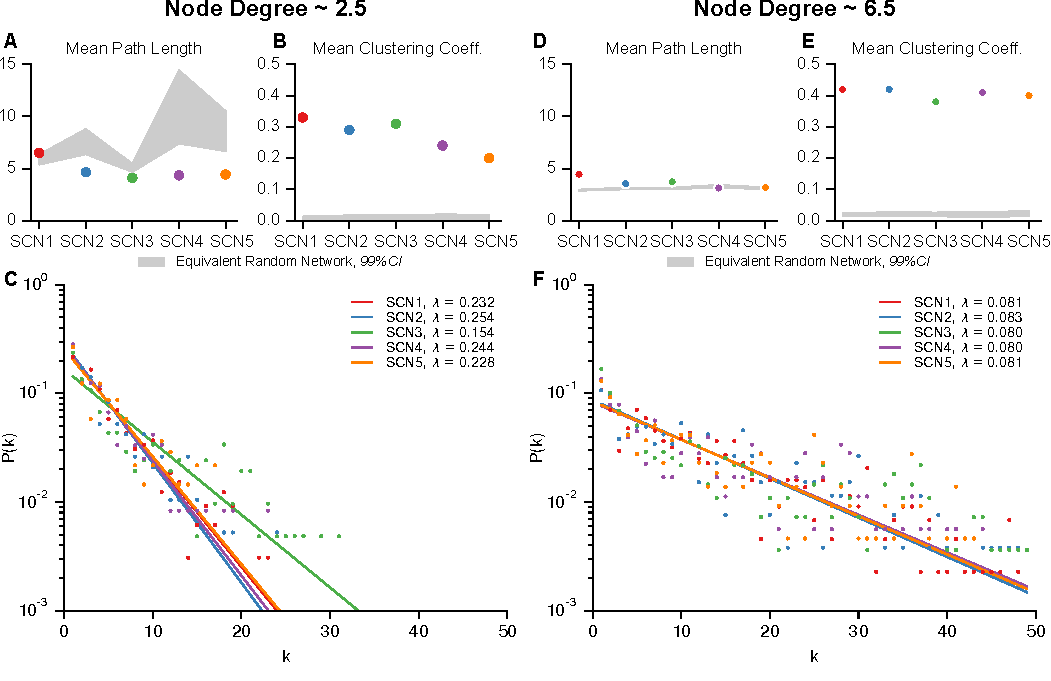
\includegraphics[width=6.5in]{chap3/figures/s5.pdf}
    \end{center}
    \caption{\label{fig:s5} Small-world network characteristics and discrete exponential distribution of node degree is insensitive to selected MIC threshold. Threshold was altered for each SCN to yield an average node degree of approximately 2.5 (A-C) and 6.5 (D-F). (\textbf{A},\textbf{D}) Average path length remains on the same order of magnitude as that of an equivalent random network (99\% confidence interval taken from 10,000 randomly-generated networks). (\textbf{B},\textbf{E}) Average clustering coefficient remains an order of magnitude higher than that of an equivalent randomly-generated network, confirming small-worldness. (\textbf{D},\textbf{F}) Node degree distribution remains exponential for average node degrees of 2.5 and 6.5. As in Figure 4, the resulting discrete exponential distributions $P(k) = C\exp(-\lambda k)$ were fit via numerical optimization of the maximum likelihood, resulting in distribution parameters $\lambda$ for each network. Each SCN is better fit by a discrete exponential distribution than a discrete power law distribution (likelihood-ratio test, $P<0.0005$ for each SCN). SCN3 lacks sufficient resolution to lower node degree below $\sim$ 4.0, and therefore shows slight deviation in $\lambda$ for low average node degree.
}
\end{figure}




A semilog plot of the node degree distribution for each SCN is shown as Figure \ref{fig:log}.
Similarly to \cite{Freeman2013a}, our node degree distribution was best fit with a discrete exponential (geometric) distribution rather than a discrete power law (zeta or Zipf) distribution.
The discrete exponential distribution, as defined in \cite{Clauset2009}, is:
\begin{equation}
    P(k) = C\exp(-\lambda k),
\end{equation}
where the normalization constant $C$ is:
\begin{equation}
    C = (1-\exp(-\lambda))\exp(\lambda k_{min}),
\end{equation}
$\lambda$ is the inverse scale parameter, and $k_{min}$ is the lower limit on the exponential scaling.
For $k_{min} = 1$ (as in our case), the discrete exponential distribution is equivalent to a geometric distribution where the geometric ``success probability'' parameter $p=1-\exp(-\lambda)$.
The $\lambda$ parameter was fit via a numerical optimization of maximum likelihood, and the exponential distribution was found to perform better than a discrete power law distribution ($P<0.0005$ for each SCN, likelihood-ratio test) \cite{Clauset2009,Alstott2014}.
Figure \ref{fig:s5}C,F demonstrates that the exponential distribution of node degree is consistent across thresholds, with changes in $\lambda$.
Thus, we identified a consistent small-world discrete exponential functional network arising from SCN resynchronization.

\subsection*{Coupling is strongest in and between core SCN regions}
\afterpage{
\begin{figure}[p]
    \begin{center}
        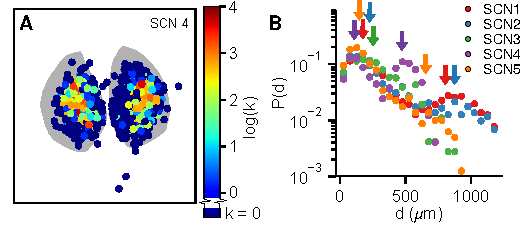
\includegraphics[width=3.5in]{chap3/figures/fig5_new.pdf}
    \end{center}
    \caption{\label{fig:dist}  Hubs of the small-world network are located in the central SCN. (\textbf{A}) Heatmap of node degree (color $\propto \log (k)$) distribution for a representative SCN shows that hubs of the small-world network are preferentially located in SCN core regions. All SCNs are shown in Figure \ref{fig:s6}.
    (\textbf{B}) Connection length ($d$ $\mu$m) distributions for SCNs 1-5 plotted on a semilog scale. Two peaks (arrows) are identifiable for SCNs 1,2,4,5: a ``local'' peak corresponding to connections between physically nearby neurons, and a second peak corresponding to the distance for functional connections between central SCN regions. For SCN3 these peaks are indistinguishable due to lack of spatial separation between cores.
}
\end{figure}


\begin{figure}[p]
    \begin{center}
        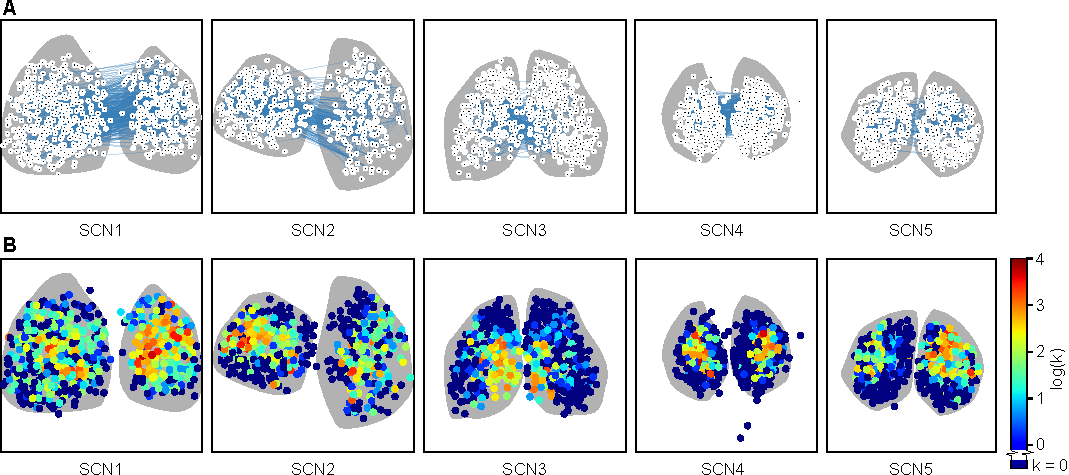
\includegraphics[width=6.5in]{chap3/figures/s6.pdf}
    \end{center}
    \caption{\label{fig:s6}
    Hubs of the small-world network are located in the central SCN. 
    (\textbf{A}) Inferred networks are shown overlaid on SCN tissue shape (gray). Connections between nodes are particularly dense in core regions and individual connections are difficult to distinguish. The 3rd ventricle is oriented at the top of each network. Strong functional connections between halves indicate that the core regions communicate to establish consistent phase to entrain the shell. Cells which have no or few functional connections are preferentially located in the outer SCN shell regions.
    (\textbf{B}) Heatmaps of node degree (color $\propto \log (k)$) distribution show that hubs of the small-world network are preferentially located in SCN core regions.
}
\end{figure}
}


Commonly, studies of the SCN have revealed two clusters of cells: a ventral core region defined by excitatory (phase attractive) GABAergic connections, VIP production, and light input from the retinohypothalamic tract \cite{Albus2005, Evans2013, DeWoskin2015, Welsh2010}.
To examine how this core-shell paradigm relates to the functional network, we examined the spatial hierarchy of the network.
Figure \ref{fig:dist}A illustrates the spatial hierarchy of node degree distribution across a representative SCN.
A lower node degree was observed in the shell region, relative to the higher node degree generally seen in the SCN core, obtained by our inference method. 
We note that in each SCN, a number (average 45\%) of cells in the SCN displayed no functional connections.
These cells are primarily located in the shell regions (Figure \ref{fig:dist}A).
This does not indicate that there are no physiological connections, since shell neurons do resynchronize with the rest of the SCN.
More likely, connections in this region are weaker and insufficient to rapidly resynchronize these cells above our functional connection MIC threshold.
This structure is consistent even when accounting for phase lags between individual cells within the fully synchronized SCN (see Figure \ref{fig:s4} following the main results).
Strikingly, this result of one cluster and the \textit{absence} of a second cluster differs from prior studies of the functional organization of the SCN, which identified two phase clusters of neurons \cite{Evans2013}.


The distribution of functional path distances ($d$) is shown in Figure \ref{fig:dist}B.
The functional path distance is defined as the physical separation between two functionally-connected cells.
This distribution also appears exponential for each network, where the likelihood of a connection existing at distance $d$ exponentially decays with this $d$.
These distributions are not strictly unimodal, rather, SCNs 1, 2, 4, and 5 display a second peak (identifiable via continuous wavelet transform peak detection) which corresponds to the physical separation between core regions.
SCN3 lacks this second peak as the identified cores of each half lack spatial separation.
The presence of this second peak indicates that core-core functional connections within a SCN are more prominent than average long-range functional connections.
Furthermore, it indicates that core-core coupling is tighter than core-shell coupling.


\subsection*{Relationship between physical and functional networks via network resimulation}

Since the physical connections between cells cannot be directly probed, we focused on obtaining the \textit{functional} network structure.
Here, we simulated the TTX experiment using stochastic circadian oscillator networks (using models from \cite{Gonze2006, Schroder2012, Abel2015a}) to determine how the functional network we infer is related to the underlying physical connectivity in the SCN.
First, we tested the efficacy of this method for inferring simulated physical networks of 400 cells with either linear nearest neighbor, small world Watts-Strogatz \cite{Watts1998}, or random network topology.
Next, we simulated the networks we inferred from SCN slices and show that our method can re-infer these physical networks with good accuracy.
Details regarding these simulations are included in the Supplement.

In Figure \ref{fig:s7}, we show representative traces from these simulations and further demonstrate that our method is able to recapture the underlying physical networks (random, Watts-Strogatz small-world, nearest neighbor) with accuracy dependent on the density of connections.
Functional networks inferred via our resynchronization and MIC method do not accurately recapture physical networks with dense random structure, as secondary indirect connections between nodes may be functionally identified as direct connections.
To validate the consistency of specific network structures inferred from TTX experiments, we simulated the SCN networks discovered in the previous section and again inferred the network from these simulations.
The resynchronization-MIC method performed well in recapturing simulated SCN networks, with an average area under the ROC curve (AUC) of $0.94$ for the three-state model and $0.80$ for the more complex eleven-state model.
The ROC curves are plotted for each SCN in Figure \ref{fig:s8}.
We note that the false positives are most often incurred in distinguishing between primary and secondary connections within dense regions, while disconnected nodes are easily identified.
Thus, this methodology can distinguish well between regions with dense and sparse physical connections such as the core and shell, but is less apt at identifying the individual physical connections in each region.
\begin{figure}[p]
    \begin{center}
        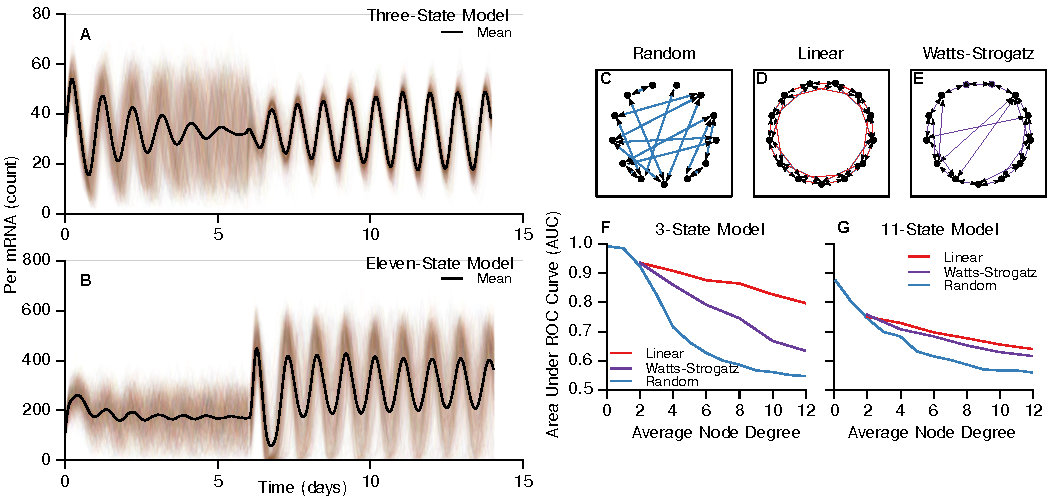
\includegraphics[width=6.5in]{chap3/figures/s7.pdf}
    \end{center}
    \caption{\label{fig:s7}
    Accuracy of the MIC inference method depends on both network topology and average node degree. 
    (\textbf{A}) and (\textbf{B}) show representative simulations capturing the TTX-mediated resynchronization for the three-state and eleven-state models, respectively.
    Next, MIC network inference was performed for simulated networks of three topologies: (\textbf{C}) random, (\textbf{D}), linear nearest neighbor, and (\textbf{E}) Watts-Strogatz small world ($\beta=0.05$).
    These networks are only shown for visualization of network structure.
    Simulated networks each contained 400 cells to match SCN recordings, and the average AUC was calculated for 5 dynamically-generated networks of each node degree.
    The area under the ROC curve is plotted as a function of average node degree for the three-state circadian model \cite{Gonze2006,Schroder2012} (\textbf{D}) and the eleven-state circadian model \cite{Abel2015a} (\textbf{E}) for these network structures.
    We show that both node degree and network structure affect the accuracy of this method.
    In general, networks that have a shorter average path length and higher average node degree are more difficult to accurately infer, as it becomes increasingly difficult to differentiate between direct and indirect physical connections.
}
\end{figure}

\begin{figure}[p]
    \begin{center}
        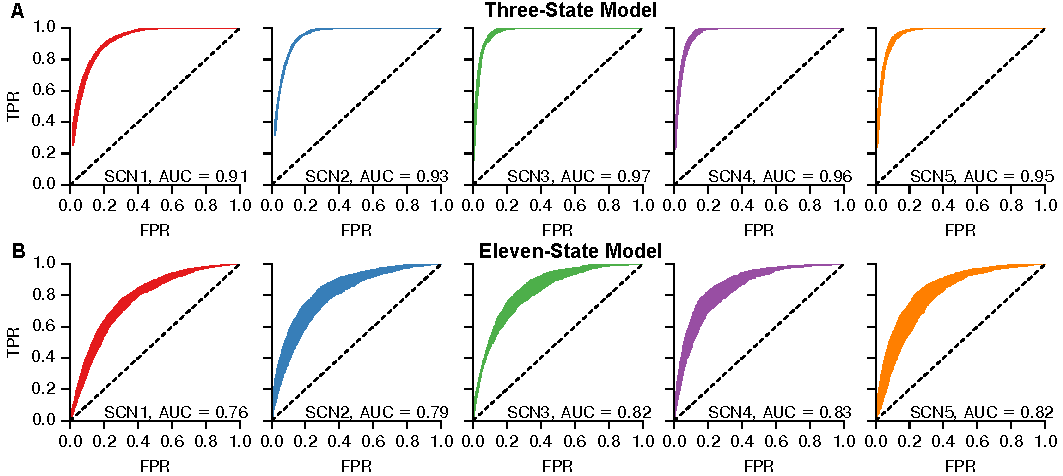
\includegraphics[width=6.5in]{chap3/figures/s8.pdf}
    \end{center}
    \caption{\label{fig:s8} Receiver operating characteristic (ROC) curve ranges and mean AUC values for simulation and inference of the SCN networks with physical connections dictated by the functional network, using (\textbf{A}) the three-state \cite{Gonze2006,Schroder2012} and (\textbf{B}) the eleven-state \cite{Abel2015a} models. Shaded ranges were calculated from 7 simulations using unique random seeds. We note that all neurons are simulated, including those which are unconnected. Unconnected neurons do synchronize experimentally though at a slower rate. To reflect this, unconnected cells in simulation were connected to the mean field, but at a reduced coupling strength. Errors in this method are largely incurred by secondary connections within tightly coupled regions (i.e. physical connections of cell 1 $\rightarrow$ cell 2 $\rightarrow$ cell 3 often show the additional cell 1 $\rightarrow$ cell 3 functional connection). Thus, we may understand that errors are incurred by functional connections in regions of dense physical connectivity appearing more dense.
}
\end{figure}




\begin{figure}[p]
    \caption{\label{fig:s4}
Effect of phase offset on MIC network inference.
    MIC is not phase-agnostic, and so the question arises of whether the inferred functional networks are driven by phase distributions in each SCN, similar to the phase clusters identified in \cite{Evans2013}.
First, we show how phase offset affects MIC score for pairs of synchronized oscillators.
Next, we show that re-aligning out of phase trajectories and taking the maximum MIC reduces much of this bias.
Finally, we examine how this affects the connections we identify in the five SCN tissues, and show that our results are consistent after applying this phase offset correction.
    (\textbf{A})
    The MIC score varies with phase offset between two phase-locked oscillators.
    Each point on this plot was generated by simulating 50 pairs of strongly coupled cells, as in S2.
    Connected cells in this model synchronize to a phase offset of 0h because they are parameterized identically.
    One trajectory from each pair was phase-shifted in 0.1h increments up to 12h, to generate a range of phase offsets between the trajectories.
    The mean MIC score (y-axis) of the 50 pairs was then computed for each artificially-created phase offset (x-axis).
    As the phase offset between coupled cells is increased, the MIC score is reduced from its maximum at a 0h angle.
    This is considered the uncorrected case, where MIC is computed with no regard for the phase offset between trajectories.
    (\textbf{B})
    Next, we took the phase-shifted trajectories from (A) and performed a correction to renormalize MIC, so that MIC score is not affected by the phase offset between cells which we originally added.
    The correction was performed by again shifting the trajectories 12h in either direction, this time in intervals of 1.0h to reflect experimental sampling rate, and calculating MIC scores at each of these shifts.
    We then selected the largest of the resulting values as the MIC score for the cell pair, as this maximum MIC corresponds to when phases are realigned.
    In comparison to the uncorrected method, the maximum MIC correction results in reduced sensitivity to the phase offset between cells, as the corrected MIC score (y-axis) is nearly flat with respect to the phase offset of the pair (x-axis).
    This method reduces power however, as some of the initial resynchronization period must be truncated in order to realign phases, resulting in a slight bias toward \textit{larger} phase offsets.
    Thus, the uncorrected method (biased toward small phase offset) and corrected maximum MIC method (slightly biased toward large phase offset) form bounds on connectivity.
    (\textbf{C}) Scatter plot of MIC score vs. mean phase offset for all possible connections within each SCN.
    There is a clear bias against absolute phase offsets greater than $\sim2$h (left), in a similar form to (A).
    This bias is rectified by performing the maximum MIC correction (right).
    Phase offset (used only for plotting purposes) was calculated by a Hilbert transform after removing the trend via discrete wavelet baseline detrending.
    As the phase offset was unstable early during resynchronization, it was calculated after it had stabilized, during days 6-7.
}
\end{figure}

\begin{figure}[p]
\contcaption{(Continued.)
        (\textbf{D}) Plot of standard deviation of phase offset vs. mean phase offset for possible and identified connections within all five SCNs.
    Standard deviation of phase offset was calculated throughout the resynchronization period, and can be thought of as a measure of phase offset instability between two cells.
    As expected, MIC detects connections between cells with a low standard deviation in phase offset for both cases, with a wider range of mean phase offsets .
    Thresholds were raised for each of the five SCNs (to 0.980, 0.970, 0.999, 0.985, 0.985 respectively) after phase correction, as all MIC scores are increased by this method.
    Generally, cell pairs with a larger phase offset also had a less stable phase offset, such that even after phase offset correction most connections were between cells with an difference in phase of less than 2h.
    (\textbf{E}) Phase-corrected SCN networks maintained small-world characteristics, with a comparable mean path length and larger clustering coefficient than corresponding random networks.
(\textbf{F}) Node degree distributions for each SCN remain exponential (P<0.0001 for each SCN, likelihood-ratio test comparison with power law fits), though $\lambda$ changes corresponding to the increased average node degree for SCNs in which phases were aligned.
    SCN 3 deviates slightly from the others here, due to the high number of connections which yield saturated (1.0) MIC scores after re-alignment.
    (\textbf{G}) Connection length distributions for unaligned and phase-aligned networks. 
    Despite the higher average node degree for aligned networks, these distributions continued to display two peaks: one for local connections within a core, and a second corresponding to core-core connections.
(\textbf{H}) Similarly, core-shell hierarchy was maintained after phase-alignment. Additionally, many shell neurons remain functionally ``unconnected,'' indicating a much slower resynchronization than neurons in SCN core regions.
    These neurons do synchronize, however, they are less tightly synchronized than cells which have identifiable connections.}
\end{figure}

\begin{figure}[p]
    \begin{center}
        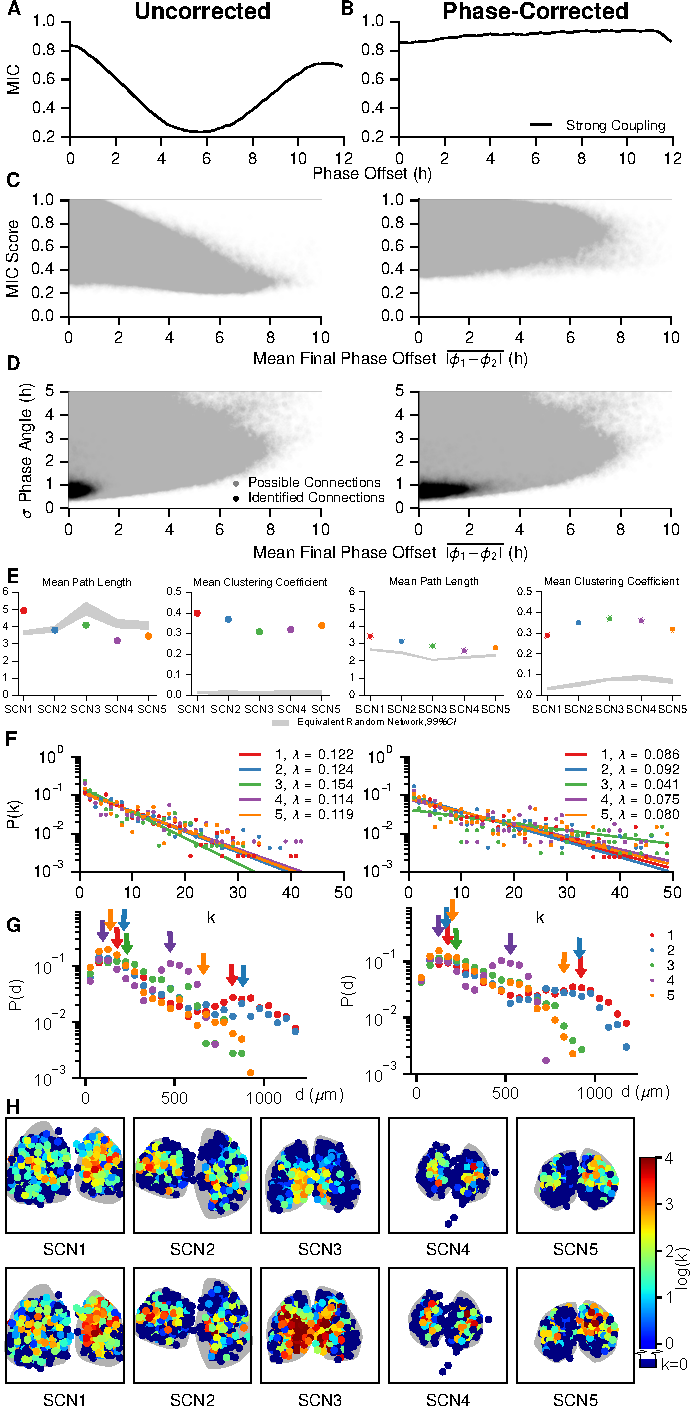
\includegraphics[width=4.15in]{chap3/figures/s4_new.pdf}
    \end{center}
\contcaption{(Continued.)}
\end{figure}

\section{Discussion}

In this work, we inferred the functional network of the suprachiasmatic nucleus during resynchronization through the use of a TTX-mediated resynchronization and the maximal information coefficient.
The functional networks we found were consistent across all samples, displaying small-world characteristics, a discrete exponential node degree distribution, and core-shell spatial hierarchy in which densely functionally-connected cores synchronize rapidly.
Our results are consistent with previous studies which show differences in function and neurotransmitter activity between core and shell SCN neurons \cite{Albus2005, Yan2005, Evans2011, Evans2013, Watanabe2007, Welsh2010, Evans2015, Myung2015, DeWoskin2015}.
However, in this work for the first time we probe connectivity within these clusters.
This leads to two surprising results: a lack of a second functionally connected cluster in the shell region, and dense connections between SCN cores.

It is well-established that exposure to artificial long day or light:dark:light:dark frequency doubling conditions can split the SCN into core and shell phase clusters, which oscillate with a large phase lag and also result in behavioral splitting \cite{Watanabe2007,Evans2011,Evans2013}.
Although shell neurons form a phase cluster under these conditions, we found few functional connections within this region even when accounting for phase alignment, suggesting that the phase clustering is driven by a common response to light reception and mediated by the core SCN rather than driven by tight connectivity within the shell itself.
This is one particular advantage of the TTX assay we employ: light-based approaches are unable to differentiate between cells which have identical responses to a common stimulus, and cells which communicate to establish similar behavior.
A previous study of SCN reentrainment to shifted light exposure also showed that the ventral SCN reentrained rapidly, while the dorsal region took several days to reentrain \cite{Albus2005}.
It was proposed that the core entrained rapidly due to its receiving input from the retinohypothalamic tract (RHT), and showed that synchronization of the shell was mediated by the effect of excitatory GABA.
As our resynchronization conditions are chemically-induced and do not involve light input, it was unexpected that a fast-resynchronizing core/slow-resynchronizing shell is a conserved feature between these studies.
This consistency indicates that the underlying structure of the SCN, rather than simply RHT connection, drives the dominant role of the core SCN.

We did not attempt to identify connection directionality or the molecular mechanisms driving connectivity, and it is possible that multiple pathways are involved.
It has been shown that excitatory GABA action drives reentrainment of the shell region in response to light phase shifts \cite{Albus2005}.
This was examined in depth in recent collaborative works \cite{Myung2015, DeWoskin2015}; these studies demonstrated the encoding of day length through the GABA pathway, by the Cl$^-$-dependent excitatory (core, phase-attractive) or inhibitory (shell, phase-repulsive) effects of slow-scale (tonic) GABA.
Visually, the core regions identified in our networks overlap with the regions of excitatory GABA action \cite{Myung2015}.
In future studies, our TTX-based assay could be combined with VIP/GABA/glutamate agonist or antagonist application and repeated in order to identify the molecular mechanisms responsible for the identified connections.
If GABA coupling affects differentiation between core hub neurons and shell neurons, this would result in significant seasonal plasticity of the functional network.

The functional networks we inferred contained a surprising number of connections between core regions of each suprachiasmatic nucleus.
The SCN is often thought to be most tightly connected within each half, given the ability of the left and right SCN to oscillate in antiphase in animals exposed to constant light \cite{Delaiglesia2000, Ohta2005}.
However, tight bilateral coupling is reflective of previous studies which showed significant coupling between the halves and further implicates the glutamate receptor in this communication \cite{Michel2013}.
This is especially interesting, since the glutamate receptor has also been implicated in communication between the SCN and the RHT, which occurs in the core SCN region \cite{Ebling1996}.
Thus, our results support the hypothesis that antiphasic oscillation between SCN halves in constant light is made possible by distinct signalling mechanisms in the SCN rather than a weaker coupling strength between halves \cite{Indic2008, Michel2013}.
It is unclear if connections between halves are synaptic or diffusive.

Theoretical studies in network science as well as modeling studies specific to the circadian field have pointed to possible advantages and causes of a small-world network structure.
Small-world exponential networks provide advantages in robustness due to having ``hubs'' of high node degree and many less-important nodes of low node degree.
Networks with this topology are better able to maintain short paths of communication when randomly-selected nodes are removed \cite{Albert2002}, due to the redundancy and long-range connections provided by network hubs.
This could occur during aging, as it is known that some brain regions lose mass during the aging process.
Small-world topology has also been shown to enhance synchronization and amplitude properties of the SCN with a lower energy cost (fewer connections) when compared to random and nearest-neighbor networks \cite{Vasalou2009, Hafner2012}.
Theoretical studies have predicted that spatially embedded small-world networks, such as neuronal networks, would display an exponential node degree distribution as seen in our data \cite{Ozik2004, Zitin2014}.
This distribution would result from growth of a small initial population of connected nodes.
As more nodes are added, the neuron population is forced to move spatially and initial local connections ultimately become long-range, while new short-range connections form.
In this context, it is striking to note that the fetal SCN forms as neurons are added to the core first and then shell regions. The connections we measure, therefore may reflect the ontogeny of synapse formation in the SCN. 
If, however, core-core long range connections are found to be diffusive rather than synaptic, this hypothesis would not apply.
Future experiments could test whether the left and right SCN must form synapses to synchronize, for example, in co-cultures.

Our work presents both a new perspective on connectivity within the SCN and a new assay for observing communication between individual circadian neurons at high spatial resolution.
A major difficulty in mapping the SCN and the brain as a whole lies partly in the multiple time and physical scales at play.
One method alone is insufficient to map the whole SCN at all resolutions, necessitating multiple perspectives to achieve spatial, directional, and mechanistic specificity.
In conjunction with light-driven desynchronization assays, antagonist/agonist application, genetic knockdowns, and mathematical modeling, this TTX assay with correlation metrics can be used to further probe connections within the SCN at a single-cell level, and between the SCN and other brain regions.

Finally, although we have presented results indicating heterogeneous network structure within the SCN, we have not proposed a means by which this structure arsises.
Studies of the onset of circadian oscillation in the fetal SCN have been limited to whole-SCN analyses, in part due to the experimental challenge of explanting the fetal SCN and recording the activity of distinct neurons.
In the ensuing chapter, we begin to approach questions of ontogeny of cell-autonomous circadian rhythms in SCN neurons, and how and when the network driving circadian synchrony arises.
Importantly, the core-shell heterogeneity of the SCN observed in this study as well as others provides a marker for a ``mature'' SCN network.



























